%!TEX root = ../notas_de_clase.tex

\section{Regresión Lineal} 

El problema de regresión busca determinar la relación entre una variable \emph{independiente} (entrada, estímulo o instancia; usualmente denotada por $x$) y una variable \emph{independiente} (salida, respuesta o etiqueta; usualmente denotada $y$). Intuitivamente, un modelo de regresión permite entender cómo cambia la variable dependiente cuando la variable independiente es modificada. Esta relación entre ambas variables es representada por una función, consecuentemente, el problema de regresión es equivalente a encontrar una función. De esta forma, en base a (i) el espacio de posible funciones donde se busque dicha relación (por ejemplo el espacio de todos los polinomios de grado menor o igual a 5), y a (ii) el criterio de búsqueda que se aplique, podemos obtener distintas soluciones para el problema de regresión. 

El escenario básico de regresión, y que sirve de base para casos más complejos, es el de regresión lineal. En este caso, el espacio de funciones donde se busca la relación entre las variables dependientes e independientes es el de las funciones lineales afines. Específicamente, para un conjunto de observaciones de $N\in\N$ entradas $\{x_i\}_{i=1}^N$ y salidas $\{y_i\}_{i=1}^N$ de la forma
\begin{equation}
	\{(x_i,y_i)\}_{i=1}^N\subset \R^M \times \R,
	\label{eq:training_set}
\end{equation}
la regresión lineal busca encontrar un modelo lineal, es decir, una función $f(\cdot)$ definida por 
\begin{align}
  f \colon \R^M &\to \R\nonumber\\
  x &\mapsto f(x)=a^\top x + b,\quad a\in\R^M,b\in\R,
 \label{eq:reg_lin_fn} 
\end{align}
que \emph{mejor represente} la forma en que la variable $y$ depende de la variable $x$, en base a las las observaciones descritas en la ecuación~\eqref{eq:training_set}. Antes de proceder a definir un criterio de \emph{mejor representación}, el siguiente recuadro analiza la elección de modelos lineales. 

\begin{mdframed}[style=discusion, frametitle={\center ¿Por qué consideramos el caso lineal en particular?}]

	Existen distintas razones para estudiar los modelos lineales. En primer lugar, con el criterio de mínimos cuadrados que veremos a continuación, el modelo lineal es el único que admite resolución de forma explícita (o, como diremos alternativamente, \emph{tiene forma cerrada}). Esto, además de permitirnos calcular dicha solución, nos permite interpretar sus propiedades y en qué casos dicha solución tiene sentido. En segundo lugar, los resultados que obtendremos a continuación requieren linealidad solo en los parámetros---ver ecuación~\eqref{eq:reg_lin_fn}---y no necesariamente en la variable independiente $x$. Por esta razón, el estudio del modelo lineal también incluye modelos no lineales del tipo
\begin{align}
  f \colon \R^M & \to \R\nonumber\\
  x &\mapsto f(x)=\theta^\top \phi(x) \quad \theta\in\R^{M'}
 \label{eq:reg_no_lin_fn} 
\end{align}
donde $\phi \colon \R^M \to \R^{M'}$ es una función no lineal sin parámetros libres. Es decir, estrictamente hablando deberíamos referirnos a los modelos lineales como \emph{lineales en los parámetros} y no necesariamente en la entrada. 

Finalmente, cuando los parámetros a determinar en el problema de regresión afectan de forma no lineal la relación entre las variables dependiente e independiente, el análisis presentado a continuación no es válido y en general la solución óptima de mínimos cuadrados no tiene forma cerrada. 

\end{mdframed}



\subsection{Mínimos cuadrados} % (fold)
\label{ssub:min_cuad}
En el contexto recién presentado, aflora naturalmente la siguiente pregunta: \emph{¿qué es una buena función $f(\cdot)$?} o, equivalentemente, \emph{¿cómo cuantificar la bondad de un modelo de regresión lineal?} Una práctica ampliamente utilizada es elegir la función $f(\cdot)$ en la ecuación \eqref{eq:reg_lin_fn} de acuerdo al criterio de \textbf{mínimos cuadrados}. Es decir, elegir la función $f(\cdot)$ que minimiza la suma de los cuadrados de las diferencias entre las observaciones $y$ y las predicciones calculadas por la función $f(x)$ de acuerdo al siguiente costo:
\begin{equation}
	J(\{(x_i,y_i)\}_{i=1}^N,f) = \frac{1}{2}\sum_{i=1}^N(y_i-f(x_i))^2,
	\label{eq:least_squares_cost}
\end{equation}
donde hemos sido enfáticos en que el costo depende del conjunto de entrenamiento $\{(x_i,y_i)\}_{i=1}^N$ y la función $f$, sin embargo, cuando estas cantidades son claras, nos referiremos al costo simplemente como $J$. Además, denotamos la (o las) funciones que satisfacen el criterio de mínimos cuadrados mediante\footnote{La constante $\frac{1}{2}$ que multiplica al costo cuadrático no afecta la solución y está ahí por simplicidad de notación cuando se calculen las derivadas de esta expresión.} 
\begin{equation}
	f^\star = \argmin_{f\text{ es lineal}} J.
\end{equation}
Debido a la forma lineal de $f(\cdot)$, resolver este problema de optimización es equivalente a encontrar los parámetros $a$ y $b$ en la ecuación ~\eqref{eq:reg_lin_fn}. Es decir: 
\begin{equation}
	a^\star,b^\star = \argmin_{a,b} \frac{1}{2}\sum_{i=1}^N(y_i-a^
	\top x_i + b)^2.
	\label{eq:lin_least_squares}
\end{equation}

Observemos que el costo en la  ecuación \eqref{eq:lin_least_squares} es cuadrático en $a$ y $b$, por lo el problema de optimización tiene un único mínimo que puede ser encontrado explícitamente. Para esto, como la función $f$ en la ecuación~\eqref{eq:reg_lin_fn} no es lineal sino que \emph{afín}, hacemos el siguiente cambio de variable:
\begin{equation}
  \left[ \begin{matrix}x \\  1\end{matrix}\right] \mapsto \tx\in\R^{M+1},\quad
  \left[ \begin{matrix}a \\  b\end{matrix}\right]\mapsto \theta\in\R^{M+1},
 \label{eq:truco_reg_lin} 
\end{equation}
con lo cual el funcional cuadrático a minimizar se convierte en
\begin{equation}
	J = \frac{1}{2}\sum_{i=1}^N(y_i-\theta^
	\top \tx_i)^2,
	\label{eq:lin_least_squares2}
\end{equation} 
y el parámetro $\theta$ de mínimos cuadrados puede ser encontrado aplicando las condiciones de primer orden de la siguiente forma:
\begin{align}
\nabla_\theta J=0 &\Leftrightarrow \sum_{i=1}^N(y_i-\theta^\top \tx_i)\tx_i^\top=0  							&&\text{def. $J$}\nonumber\\  
&\Leftrightarrow \sum_{i=1}^Ny_i\tx_i^\top = \sum_{i=1}^N\theta^\top \tx_i\tx_i^\top					&&\text{ordenar}\nonumber\\
&\Leftrightarrow \theta^\top = \sum_{i=1}^Ny_i\tx_i^\top \left(\sum_{i=1}^N \tx_i\tx_i^\top\right)^{-1}	&&\text{despejar $\theta^\top$}\nonumber\\
&\Leftrightarrow \theta =  \left(\sum_{i=1}^N \tx_i\tx_i^\top\right)^{-1} \sum_{i=1}^N \tx_i y_i 		&&\text{transponer}\nonumber\\
&\Leftrightarrow \theta = \left(\tX^\top\tX \right)^{-1} \tX^\top Y, 											&&\text{def. $\tX$ y $Y$} \label{eq:sol_mse}
\end{align}
donde $\tX$ y $Y$ son las matrices de datos definidas por

\begin{equation}
  \tX = \left[ \begin{matrix}\tx_1^\top \\\vdots \\ \tx_N^\top \end{matrix}\right]\in\R^{N\times (M+1)} ,\quad
  Y = \left[ \begin{matrix}y_1 \\\vdots \\y_N \end{matrix}\right] \in\R^{N}.
 \label{eq:matrices_X} 
\end{equation}

Con los parámetros del modelo regresión lineal encontrados con el criterio de mínimos cuadrados, es posible implementar la solución y comprarla visualmente con los datos. La Figura \ref{fig:reg_lin_1} muestra esta visualización de la regresión lineal para observaciones correspondientes a chirridos de grillos por segundo en función de la temperatura \cite{insects}. 

\begin{figure}[H]
	\centering
	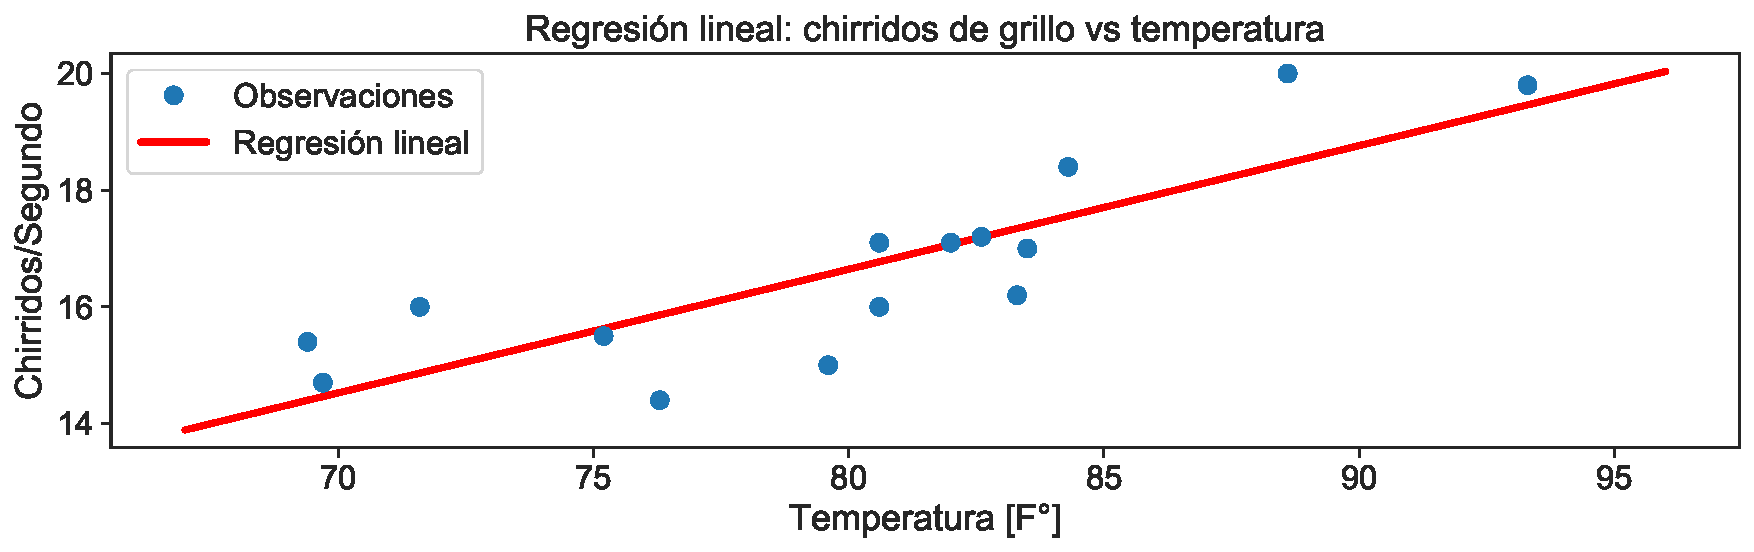
\includegraphics[width=0.9\textwidth]{img/cap1_chirridos.pdf}\\
	\caption{Ejemplo de regresión lineal.}
	\label{fig:reg_lin_1}
\end{figure}

La expresión $\left(\tX^\top\tX \right)^{-1} \tX^\top$ en la ecuación~\eqref{eq:sol_mse} es conocida como la pseudo-inversa de Moore-Penrose \cite[p.~7]{benisrael_greville_2006}. Observe que una condición \textbf{necesaria} para que esta pseudo-inversa esté bien definida es que la cantidad de observaciones ($N$) sea mayor o igual que la cantidad de dimensiones ($M+1$). Esto es porque la matriz $\tX^\top\tX$ es de tamaño $(M+1)\times(M+1)$ y su rango es $\min \{N, M+1\}$, consecuentemente, para que $\tX^\top\tX$ tenga rango completo (y por ende sea invertible), se debe cumplir al menos que $N\geq M+1$. Adicionalmente, una condición \textbf{necesaria y suficiente}  para la existencia de la solución de mínimos cuadrados en la ecuación \eqref{eq:sol_mse}, requiere que las $N\geq M+1$ observaciones\footnote{Recordemos que nos referimos a las observaciones aumentadas $\tilde{x}$} sean linealmente independientes, pues de esta forma los términos que componen la pseudo-inversa son efectivamente linealmente independiente y ésta tiene rango completo. Es claro que para el caso de variables continuas es muy poco probable que dos observaciones sean perfectamente colinearles, sin embargo, en el caso de variables categóricas donde las observaciones son asignadas a un número finito de símbolos es probable que dos o más valores para la variable dependiente sean exactamente iguales. 

En la práctica, es usual que tengamos más observaciones que parámetros al considerar un modelo lineal y que estas sean linealmente independientes. Sin embargo, es posible que las observaciones sean tal que la inversión de la matriz  $\tX^\top\tX$ sea numéricamente  inestable. Esto ocurre fundamentalmente en dos casos ilustrados en el siguiente recuadro.  

\begin{mdframed}[style=discusion, frametitle={\center ¿Matriz cuasi-singular o incorrectamente escalada?}]

Al tratar de invertir una matriz de forma computacional, probablemente hemos obtenido un mensaje de la forma \emph{Matrix is singular, close to singular or badly scaled}. Veremos dos ejemplos para entender de dónde viene esta advertencia. 

\noindent\textbf{Caso 1:} Consideremos la matriz 
\begin{equation}
	A = \left[ \begin{matrix}10^{50} & 1 \\  10^{50}  & 2\end{matrix}\right]
\end{equation}
dicha matriz es claramente invertible y su inversa puede ser calculada mediante
\begin{equation}
	A^{-1} = \frac{1}{10^{50} \cdot 2 - 10^{50}\cdot 1}\left[ \begin{matrix}2 & -1 \\  -10^{50}  & 10^{50}\end{matrix}\right]
	=\left[ \begin{matrix}2\cdot10^{-50} & -10^{-50} \\  -1  & 1\end{matrix}\right],
\end{equation}
donde cuyos elementos difieren en 50 órdenes de magnitud. Sin embargo, la representación usual que consideramos cuando programamos es la de punto flotante de precisión simple, la cual considera el menor valor (de magnitud mayor que cero) de $2^{-127}\approx 10^{-38}$. Consecuentemente, los valores más pequeños que este límite serán aproximados por el elemento más cercano, es decir, cero. Utilizando la inversa aproximada, denotada $\tilde{A}^{-1}$, resulta en errores como el siguiente:
\begin{equation}
	A\tilde{A}^{-1} = \left[ \begin{matrix}10^{50} & 1 \\  10^{50}  & 2\end{matrix}\right] \left[ \begin{matrix} 0 & 0 \\  -1  & 1\end{matrix}\right] = \left[ \begin{matrix} -1 & 1 \\  -2  & 2\end{matrix}\right]
\end{equation}

\noindent\textbf{Caso 2:} Consideremos
\begin{equation}
	A = \left[ \begin{matrix} a  & a \\  b  & b + \epsilon\end{matrix}\right]
\end{equation}
la cual también es invertible para $a,\epsilon>0$, pues su determinante está dado por
\begin{equation}
	\det{A} = a(b+\epsilon) - ab = a\epsilon>0,
\end{equation}
sin embargo, si $\epsilon\ll1$ entonces el cálculo de la inversa puede sufrir inestabilidades numéricas como en el caso anterior. Sin embargo, observe para un $\eta>0$ suficientemente grande, la matriz $A+\eta I$ puede tener un determinante arbitrariamente grande (ver Sección \ref{ssub:min_cuad_reg}).
\end{mdframed}

Adicionalmente, es importante reflexionar por qué consideramos mínimos cuadrados como la métrica de error relacionada al problema de regresión. Existen varias razones por que lo hacemos, tanto técnicas como conceptuales, como también diversas desventajas de este criterio que es importante identificar. 

Desde del punto de vista técnico, el costo convexo de un modelo lineal (en los parámetros) define un problema de optimización que también es convexo y por ende tiene una solución única. Además, en el caso particular del costo cuadrático, este óptimo puede ser determinado de forma explícita (lo cual es fuertemente deseado), pues está dado únicamente por la inversión de una matriz y no mediante, e.g., una búsqueda iterativa.

Adicionalmente, desde un punto de vista conceptual, otra justificación para usar la medida del  error cuadrático es que éste representa la varianza muestral. Es decir, si considerásemos  $x$ e $y$ en la formulación del problema de regresión como variables aleatorias (VAs), entonces el error cuadrático (relacionado con la función $f$) definido por
\begin{equation}
	e= \sum_{i=1}^N (y_i-f(x_i))^2,
\end{equation}
es la varianza muestral de la variable aleatoria $y-f(x)$, lo que corresponde al \emph{error} de estimación. De igual forma, la varianza de la suma de múltiples variables aleatorias (pensemos en errores acumulados, los cuales son independientes) corresponde a la suma de las varianzas de dichas VAs. Esto ocurre precisamente cuando usamos el exponente igual a 2, y no si usáramos 1.95 o 2.05. 

Podemos además justificar el uso del error cuadrático con una motivación geométrica. Observemos que el problema de regresión (lineal) requiere encontrar una solución aproximada de un sistema lineal sobredeterminado dado por 
\begin{equation}
	\tX \theta = Y,
\end{equation}
donde la cantidad de incógnitas ($M+1$) es ampliamente superada por el número de ecuaciones ($N$). Como esta solución, desde el punto de vista de un sistema lineal, no existe, uno puede proceder a encontrar la solución para $\theta$ que reporta \emph{la menor discrepancia} entre ambos lados de la ecuación anterior. En este sentido, podemos identificar el espacio formado por todos los posibles valores que toma la combinación lineal $\tX \theta$ para distintos valores de $\theta\in\R^{M+1}$, es decir, el \emph{span} de todas las columnas de $\tX$ (los datos) definido como el \emph{espacio de las columnas de} $\tX$ o, simplemente, $\text{span}(\tX)$. Luego, podemos identificar el elemento de dicho espacio que está más cerca de $Y$  como la proyección del propio $Y$ en $\text{span}(\tX)$. Esto está ilustrado en la Figura \ref{fig:projection}, donde la condición para identificar dicha proyección es  precisamente que el vector error $\tX \theta- Y$ sea ortogonal a todo el espacio generado por los datos (de entrada) $\text{span}(\tX)$, consecuentemente, ocupando el producto interno tenemos que 
\begin{equation}
	(\tX \theta- Y)^\top \tX = 0,
\end{equation}
lo cual nos lleva directamente a la solución de mínimos cuadrados. 

\begin{figure}[t]
	\centering
	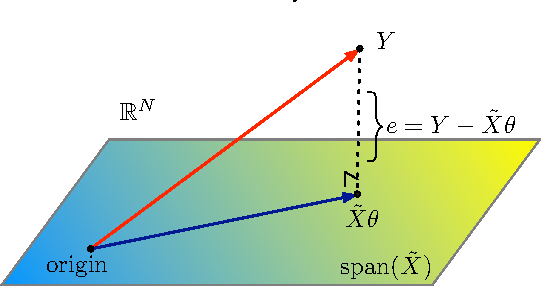
\includegraphics[width=0.5\textwidth]{img/LinRegGeo.pdf}\\
	\caption{Interpretación geométrica de la regresión lineal y mínimos cuadrados}
	\label{fig:projection}
\end{figure}

Finalmente, notemos que el criterio de  mínimos cuadrados también tiene desventajas. Implícitamente, el criterio de mínimos cuadrados está intrínsecamente relacionado con un supuesto de gaussianidad de los datos---esto será evidente cuando conectemos veamos el criterio de máxima verosimilitud---consecuentemente, el criterio de mínimos cuadrados produce estimaciones razonables cuando la relación entre $x$  e $y$ es simétrica y sin \emph{largas desviaciones}. Por el contrario, cuando existen datos  que se alejan mucho de dicha la tendencia buscada, el criterio de la suma de cuadrados puede  desviarse considerablemente de la solución buscada, esto se debe precisamente a la contribución cuadrática del error, donde, coloquialmente, una muestra \emph{muy alejada} pesa tanto o más que varias muestras \emph{ligeramente alejadas}. La Figura \ref{fig:reg_lin_2} ilustra este fenómeno para el mismo ejemplo de los chirridos en la Figura \ref{fig:reg_lin_1}, donde se ha introducido un \emph{outlier}, es decir, una observación que está inusualmente alejada de los datos y se ha recalculado el resultado de la regresión lineal mediante el criterio de mínimos cuadrados. Se puede ver cómo se deteriora la estimación solo con la introducción de un nuevo dato. 



\begin{figure}[H]
	\centering
	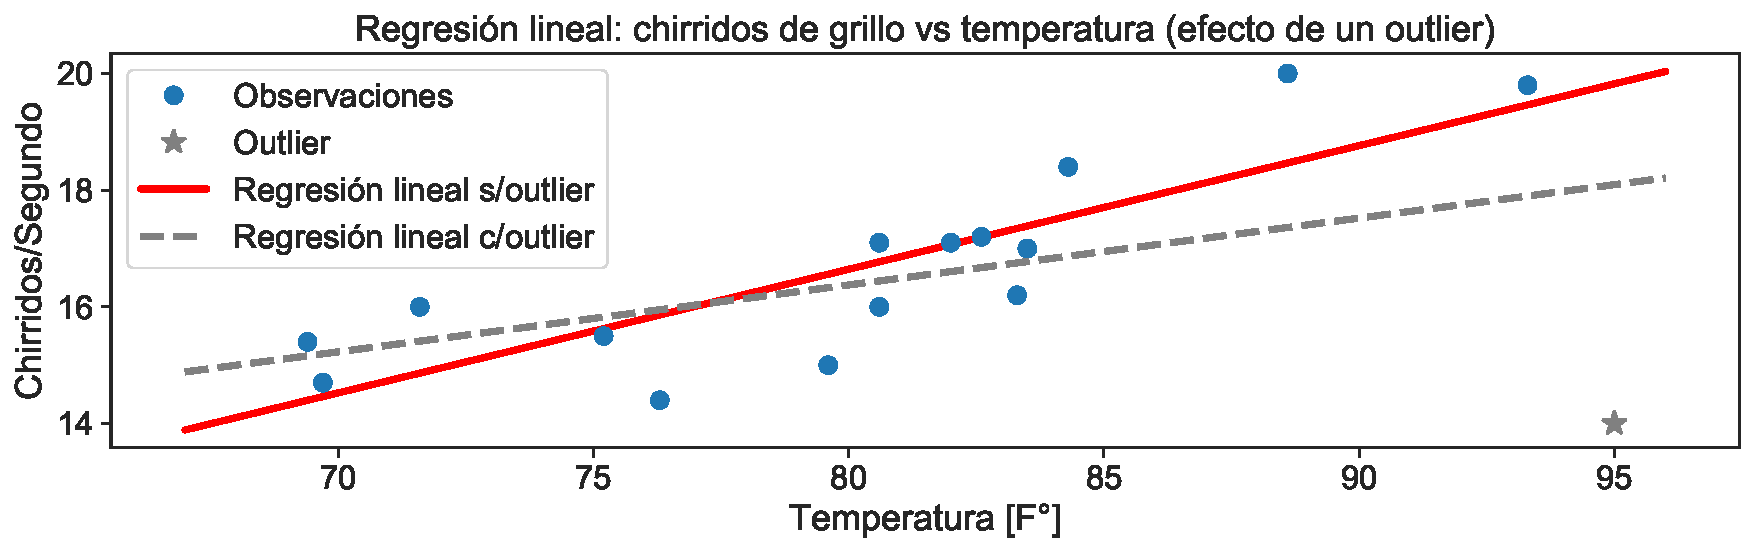
\includegraphics[width=0.9\textwidth]{img/cap1_chirridos_outlier.pdf}\\
	\caption{Efecto de un \emph{outlier} en la regresión lineal usando mínimos cuadrados: Se ha agregado un dato erróneo (\emph{outlier} en gris) y se ha recalculado la regresión lineal, note cómo la inclusión de dicho punto deteriora el resultado de la regresión.}
	\label{fig:reg_lin_2}
\end{figure}

Le lección que queda de este ejemplo es que debemos considerar una métrica \emph{ad hoc} al problema que estamos considerando, por ejemplo, si es muy probable que existan outliers, no debemos penalizar cuadráticamente los errores. De igual forma, interrogantes que es importante analizar en el momento de  elegir una métrica de error pueden tener que ver con si es irrelevante que el error de regresión sea i) cero o muy pequeño, o también ii) grande o extremadamente grande. La Figura \ref{fig:reg_lin_err} presenta cuatro métricas de error (como función del propio error), donde podemos interpretar sus propiedades. 

\begin{figure}[H]
	\centering
	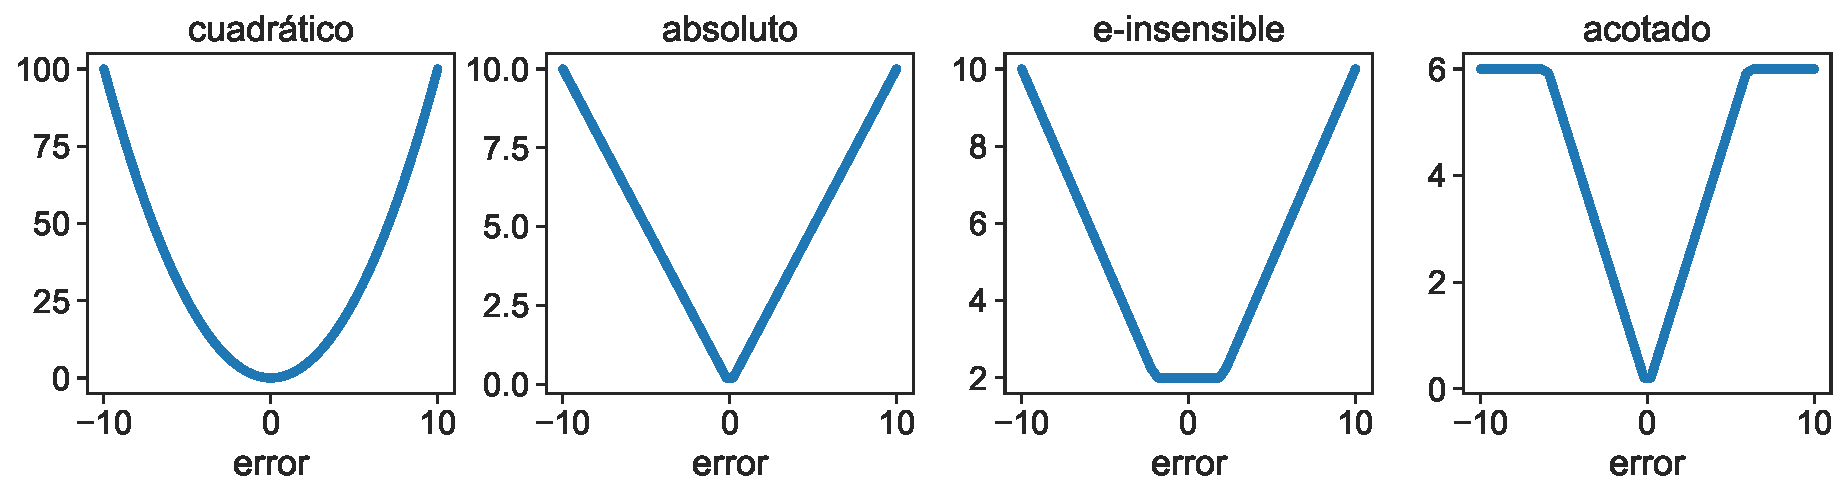
\includegraphics[width=0.8\textwidth]{img/cap1_errores.pdf}\\
	\caption{Distintas funciones de costo en función del error de estimación, de izquierda a derecha: cuadrático, absoluto (crecimiento lineal en función del error), $\epsilon$-insensible (es irrelevante si el error está entre 0 o  $\epsilon$) y acotado (es irrelevante si el error es mayor que cierto umbral).}
	\label{fig:reg_lin_err}  
\end{figure}

% subsubsection Mínimos cuadrados (end)

\subsubsection{Mínimos cuadrados regularizados} % (fold)
\label{ssub:min_cuad_reg}

Perseguir ciegamente la solución de mínimos cuadrados puede resultar, como vimos en la sección anterior, en situaciones donde la inversa de Moore-Penrose sea \emph{cercana} a singular, especialmente en los casos que las observaciones son parecidas o redundantes. En este sentido, debemos considerar un criterio que no simplemente busque un ajuste a los datos, sino que también promueva ciertas propiedades de la solución, por ejemplo, suavidad, bajas magnitudes de los parámetros o incluso pocos parámetros. Nos referiremos a estas soluciones como \emph{regulares}, en otras palabras, buscamos \emph{regularizar} la solución de mínimos cuadrados.
\iffalse
Si bien el concepto de \emph{regularizar} soluciones es uno bien  general,  en el caso de mínimos cuadrados este dice relación con  consideremos las matrices invertible $A$ y $A'=A+\rho I$ definidas mediante
\begin{equation}
	A = \left[ \begin{matrix} a  & c \\  b  & d\end{matrix}\right],
	\qquad A' = \left[ \begin{matrix} a +\rho & c \\  b  & d+\rho\end{matrix}\right]
\end{equation} 
donde $\rho>0$ y $I$ denota la matriz identidad del tamaño apropiado.   
\fi

Las penalizaciones a considerar en el problema de regresión pueden ser codificadas directamente en la función de costo. Por ejemplo, ésta puede incluir un término que penaliza el ajuste de los datos y otro término que penaliza soluciones que se alejan de lo deseado. Un criterio estándar de penalización es el basado en la norma de los parámetros, es decir, 
\begin{equation}
	J_\rho = \frac{1}{2}\sum_{i=1}^N(y_i-\theta^
	\top \tx_i)^2 + \frac{\rho}{p}||\theta||_p^p,\ p\in\R_+,
	\label{eq:reg_least_squares}
\end{equation} 
donde $||\cdot||_p$ denota la norma $\ell_p$, es decir, $||\theta||_p=\left(\sum_{j=1}^N|\theta_j|^p\right)^\frac{1}{p}$ y el parámetro $\rho\geq0$ tiene el rol de balancear la importancia entre ajuste (primer término) y regularidad de la solución (segundo término). Distintos valores de $p$ inducen distintos propiedades sobre las soluciones, siendo las más usadas las correspondientes a $p=1$, conocido como \textbf{Lasso} \cite{tibshirani_1996}, y $p=2$ conocido como \textbf{regularización de Tikhonov} \cite{tikhonov_arsenin_1977} o bien \textbf{\emph{Ridge Regression}} \cite{hoerl_kennard_1970}.  

Una ventaja de la regularización de Tikhonov es que su solución, al igual que el caso de mínimos cuadrados no regularizados, puede ser encontrada en forma exacta. En efecto, para $p=2$ el término de regularización puede ser expresado como $||\theta||_2 = \theta^\top\theta$, con lo que el minimizante del costo cuadrático regularizado está dado por: 
\begin{align}
\nabla_\theta J_\rho=0 &\Leftrightarrow \sum_{i=1}^N(\theta^\top \tx_i - y_i)\tx_i^\top + \rho\theta^\top=0  							&&\text{def. $J$}\nonumber\\  
&\Leftrightarrow \sum_{i=1}^Ny_i\tx_i^\top = \sum_{i=1}^N\theta^\top \tx_i\tx_i^\top + \rho\theta^\top					&&\text{ordenar}\nonumber\\
&\Leftrightarrow \theta^\top = \sum_{i=1}^Ny_i\tx_i^\top \left(\sum_{i=1}^N \tx_i\tx_i^\top + \rho \eye\right)^{-1}	&&\text{despejar $\theta^\top$}\nonumber\\
&\Leftrightarrow \theta =  \left(\sum_{i=1}^N \tx_i\tx_i^\top +\rho \eye\right)^{-1} \sum_{i=1}^N \tx_i y_i 		&&\text{transponer}\nonumber\\
&\Leftrightarrow \theta = \left(\tX^\top\tX +\rho \eye\right)^{-1} \tX^\top Y.								&&\text{def. $\tX$ y $Y$} \label{eq:least_sq_soln}
\end{align}

De la última expresión, es posible ver que el requerimiento de que las observaciones disponibles sean (i) más que la dimensión $M+1$ y que además (ii) éstas sean colineales ya no es necesario para que la solución esté bien definida. De hecho, la matriz $\tX^\top\tX$ puede efectivamente estar cercana a ser no invertible, sin embargo, es posible \emph{regularizar} la solución forzando que la matriz $\left(\tX^\top\tX +\rho \eye\right)$ sea efectivamente \emph{regular} aumentando el valor de $\rho$. 

En el caso de la regularización de Tikhonov, se entiende por soluciones regulares las que están definidas por parámetros que tienen una norma pequeña, tal como lo sugiere la ecuación \eqref{eq:reg_least_squares}. Sin embargo, es posible aplicar otros criterios de regularidad, por ejemplo, una solución regular puede ser una en la cual la mayoría de los de parámetros son idénticamente nulos, esto es conocido como una solución \textbf{rala} o \textbf{\emph{sparse}}. Usando por costo de regularización el número de parámetros no nulos (definido por la ``norma'' $l_0$) en la definición del costo en la ecuación \eqref{eq:reg_least_squares}, es posible determinar cuáles son las soluciones que utilizan menos variables independientes para representar la variable dependiente. Desafortunadamente, resolver encontrar la solución usando la ``norma'' $l_0$ es muy difícil, sin embargo, bajo ciertas condiciones la consideración de la norma $l_1$ puede llevar a la misma solución.

La Figura \ref{fig:reg_lin_reg} ilustra las curvas de nivel correspondientes al costo cuadrático y al  término de  regularización en la eq.~\eqref{eq:reg_least_squares} para órdenes $p\in\{0.5,1,2\}$. 

\begin{figure}[H]
	\centering
	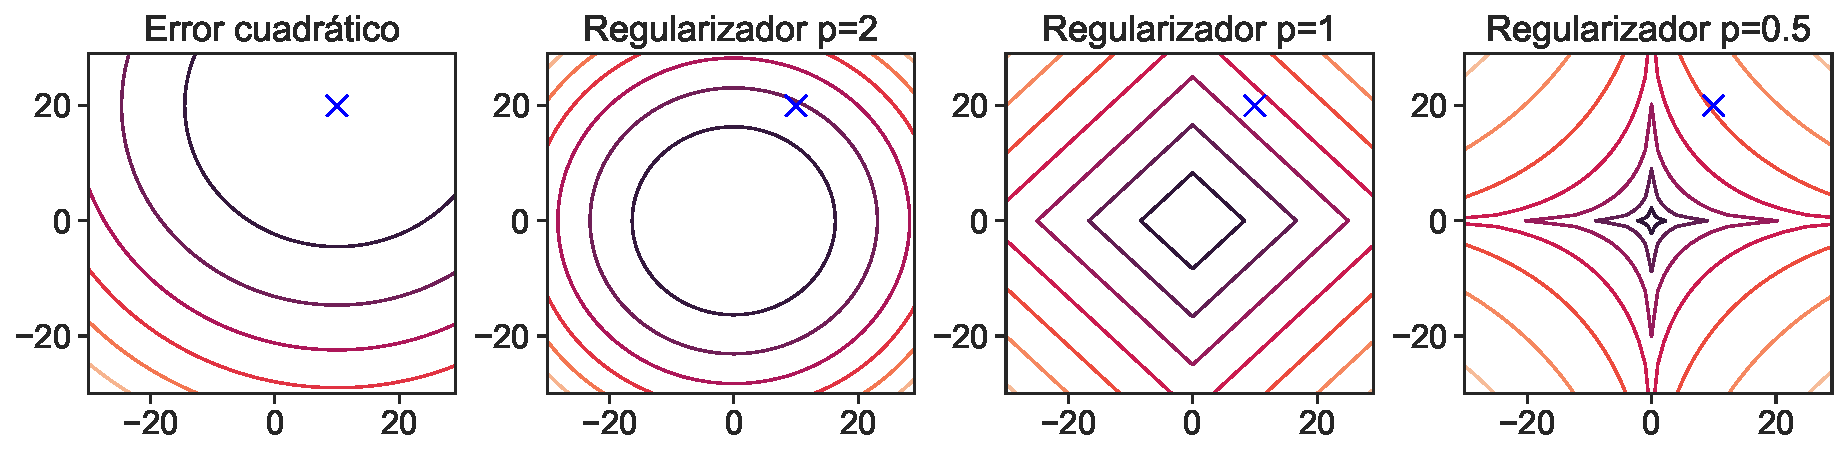
\includegraphics[width=0.8\textwidth]{img/cap1_regularizadores.pdf}\\
	\caption{Curvas de nivel del costo cuadrático para un problema hipotético con solución $\theta=[10,20]$ (izquierda) y términos de regularización para órdenes $p\in\{0.5,1,2\}$. Observe cómo las curvas de nivel atraen el mínimo hacia el origen de distinta forma: $p=2$ lleva la solución directamente al origen, mientras que $p\in\{0.5,1\}$ lleva la solución a los bordes, es  decir, privilegiando soluciones ralas. La solución $\theta=[10,20]$ se ha denotado con una cruz azul, recuerde que solo el costo cuadrático depende de este valor, no los términos de regularización. }
	\label{fig:reg_lin_reg}  
\end{figure}

\begin{mdframed}[style=pendiente, frametitle={\center Regularización versus mínimos cuadrados}]
1) Referencias, Compressed sensing, sparse feature selection\\
2) ¿es justo comprar MC y RR en términos de MSE?\\
3) Elegir el coeficiente de regularización es crítico\\
4) Notar que la regularización mueve las estimaciones de los parámetros a cero, en particular RR manda a todos \emph{igualmente} a cero, sin fijar ninguno exactamente en cero. \\
5) cuando $\rho$ es suficientemente grande, lasso puede fijar parámetros exactamente cero, consecuentemente realizando \emph{selección de variables}\\
6) formulación con restricciones\\
7) interpretación geométrica\\
8) ¿cómo elegir $\rho$? y validación cruzada: subajuste, sobreajuste
\end{mdframed}

\subsection{Máxima verosimilitud} % (fold)
\label{ssub:max_ver}

Ahora tomaremos un enfoque distinto, en el cual no buscaremos el modelo \emph{aproximado} que tiene menor discrepancia con los datos. Por el contrario, nos enfocamos en modelos que han generado \emph{exactamente} los datos observados. Debido a la naturaleza de los datos, para este fin es necesario considerar modelos estocásticos, por lo que el mejor modelo estará dado por el que \emph{más probablemente} haya generado los datos. Específicamente, consideraremos un modelo compuesto por dos partes: la primera es determinística y paramétrica (al igual que los modelos anteriores) y una parte aleatoria la cual permitirá modelar exactamente las observaciones. 

En efecto, consideremos el siguiente modelo
\begin{equation}
	y = \theta^\top\tx + \epsilon,\quad \epsilon\sim\cN(0,\sigma_\epsilon^2) \ \text{i.i.d.},
	\label{eq:lin_gauss}
\end{equation}
donde la parte determinística ha sido elegida lineal en $\tx$ y la parte aleatoria es gaussiana. El modelo probabilístico en la ecuación~\eqref{eq:lin_gauss} puede expresarse en forma distribucional como 
\begin{equation}
	y|\tx \sim p(y|\tx,\theta) = \cN(y;\theta^\top\tx,\sigma_\epsilon^2).
\end{equation}

A diferencia del criterio de mínimos cuadradros, donde el entrenamiento del modelo (ajuste del parámetro $\theta$) se hacía en base a la función de pérdida cuadrática para un parámetro dado, en este caso el criterio de entrenamiento (en función de un conjunto de observaciones) es la \textbf{probabilidad de los datos} bajo el supuesto de un modelo dado o, equivalentemente, la \textbf{verosimilitud del modelo} dado los datos. Para aclarar este criterio, y antes de considerar optimización alguna, veamos que la verosimilitud del modelo lineal y gaussiano descrito arriba está dado, para un conjunto de observaciones $T=\{(x_i,y_i)\}_{i=1}^N$, por 
\begin{equation}
	l(\theta) \deq p(Y|\tX,\theta) = p(y_1,\ldots,y_N|\tx_1,\ldots,\tx_N,\theta)= \prod_{i=1}^Np(y_i|\tx_i,\theta) = \prod_{i=1}^N \cN(y_i;\theta^\top\tx_i,\sigma_\epsilon^2), \label{eq:verosimilitud}
\end{equation} 
donde la factorización de la probabilidad de los datos es posible dado que las observaciones son \textbf{condicionalmente independiente dado el modelo}.

El ajuste del modelo entonces puede entonces realizarse mediante la maximización (con respecto a $\theta$) de la función de verosimilitud $l(\theta)$ en la ecuación~\eqref{eq:verosimilitud}. Es decir: 
\begin{equation}
	\theta^{\text{MV}}= \argmax l(\theta),
\end{equation}
donde en superíndince ``MV'' denota ``máxima verosimilitud''. 

Para el caso lineal y gaussiano presentado en la ecuación~\eqref{eq:lin_gauss}, donde recordemos que las observaciones son condicionalmente independientes dado el modelo, el estimador $\theta^{\text{MV}}$ está dado por:
\begin{align}
	\theta^{\text{MV}} 	&= \argmax \prod_{i=1}^N \cN(y_i;\theta^\top\tx_i,\sigma_\epsilon^2) \label{eq:theta_ML}\\
						&= \argmax \prod_{i=1}^N \frac{1}{\sqrt{2\pi}\sigma_\epsilon} \exp\left({\frac{-1}{2\sigma_\epsilon^2}(y_i-\theta^\top\tx_i)^2}\right) \nonumber\\
						&= \argmin \sum_{i=1}^N (y_i-\theta^\top\tx_i)^2 \nonumber
\end{align}
Nótese que es posible identificar esta última expresión con la del costo cuadrático en la ecuación \eqref{eq:lin_least_squares2}, es decir, el estimador de máxima verosimilitud es el minimizante del mismo costo que el estimador de mínimos cuadrados. Consecuentemente, ambos estimadores son iguales y de acuerdo a la ecuación \eqref{eq:sol_mse} dados por 
\begin{equation}
	\theta^{\text{MV}} = \theta^{\text{MC}} = \left(\tX^\top\tX +\rho \eye\right)^{-1} \tX^\top Y 
\end{equation}

\subsubsection{Varianza de los datos y mínimos cuadrados} % (fold)
\label{ssub:var_min_cuad}

Si consideramos el criterio de mínimos cuadrados para encontrar el parámetro óptimo en el modelo de regresión lineal, es posible determinar la varianza de los datos (con respecto al modelo lineal ajustado) mediante 

\begin{equation}
	\text{Varianza} = \frac{1}{N}\sum_{i=1}^N (y_i-\theta^\top\tx_i)^2
\end{equation}
Notemos que esta cantidad es precisamente la suma de cuadrados e intuitivamente representa la bondad de ajuste del modelo considerado. 

En el contexto de máxima verosimilitud, recordemos que la varianza es un parámetro del modelo y no una cantidad asociada al modelo que calculamos de forma independiente. Este parámetro puede ser calculado maximizando la log-verosimilitud, tal como se hizo para la media en la ecuación \eqref{eq:theta_ML}, de acuerdo a
\begin{align}
	\sigma^2_{\text{MV}} 	&= \argmax_{\sigma_\epsilon^2} \prod_{i=1}^N \cN(y_i;\theta^\top\tx_i,\sigma_\epsilon^2) \label{eq:sigma_ML}\\
						&= \argmax_{\sigma_\epsilon^2} \prod_{i=1}^N \frac{1}{\sqrt{2\pi}\sigma_\epsilon} \exp\left({\frac{-1}{2\sigma_\epsilon^2}(y_i-\theta^\top\tx_i)^2}\right) \nonumber\\
						&= \argmin_{\sigma_\epsilon^2} \frac{N}{2} \log(2\pi) +\frac{N}{2} \log(\sigma_\epsilon^{2}) + \frac{1}{2\sigma_\epsilon^2}\sum_{i=1}^N {(y_i-\theta^\top\tx_i)^2} \nonumber
\end{align}
Usando la condición de primer orden en esta expresión, tenemos que

	
\begin{align}
	\frac{N}{2\sigma^2_{\text{MV}}} - \frac{1}{2\sigma^4_{\text{MV}}}\sum_{i=1}^N {(y_i-\theta^\top\tx_i)^2} = 0 \Rightarrow \sigma^2_{\text{MV}} = \frac{1}{N}\sum_{i=1}^N {(y_i-\theta^\top\tx_i)^2}
\end{align}

Con lo cual se obtiene, sin sorpresa alguna, la misma expresión de la varianza que al usar mínimos cuadrados. La lección de este desarrollo es que, si bien tan con mínimos cuadrados o bien con máxima verosimilitud llegamos a las mismas soluciones tanto para el parámetro de la función lineal o cálculos de las varianzas, la varianza es una cantidad \emph{inherente} del modelo probabilístico y por ende puede ser calculada junto con el resto de los parámetros. 

\subsection{Regresión via inferencia bayesiana} % (fold)
\label{sub:inferencia_bayes}

En lugar de maximizar la probabilidad de que los datos hayan sido generado por el modelo propuesto para encontrar una estimación puntual del parámetro que estamos buscando, podemos calcular la distribución condicional sobre parámetros condicional a las observaciones disponibles, es decir, $p(\theta|T)$. Este criterio es conceptualmente distinto al de mínimos cuadrados o máxima verosimilitud, pues ya no nos enfocamos en encontrar el parámetro \emph{más probable} o de \emph{menor costo} sino que encontramos una distribución de probabilidad sobre el valor del parámetro que genero los datos observados. Esta distribución es conocida como \emph{distribución posterior del modelo dado los datos} y mediante el teorema de Bayes puede expresarse como

\begin{equation}
	p(\theta|T)=\frac{p(T|\theta)p(\theta)}{p(T)}
	\label{eq:posterior}
\end{equation}
donde $p(\theta)$ es la \emph{distribución a priori} del parámetro y encapsula todos nuestros supuestos, creencias y sesgo sobre el espacio de parámetros (modelos) a considerar. Finalmente, observe que la expresión de la distribución posterior tiene por denominador la \emph{distribución marginal de los datos} $p(T)$ que actúa como constante no normalización para el numerador, pues solo el numerador es función del parámetro $\theta$. Esta constante de normalización puede ser calculada mediante el uso de la ley de probabilidades totales, o bien imponiendo la restricción de que la expresión en la ecuación \eqref{eq:posterior} debe integrar uno:
\begin{equation}
	p(T) = \int p(T|\theta)p(\theta)d\theta.
\end{equation}
En base a la forma explícita de $p(T|\theta)p(\theta)$, calcular esta integral puede ser un desafío considerable. Sin embargo, enfatizamos que como esta cantidad no depende del parámetro $\theta$, no es necesario conocerla para explorar o aproximar la (forma de la) distribución posterior $p(\theta|T)$. 

La distribución posterior es entonces una \emph{mezcla} entre la distribución posterior (que representa la creencia en la variable antes de ver datos) y la verosimilitud (que representa la probabilidad de los datos condicional al modelo). Cuando la distribución a priori y a posteriori son de la misma familia, diremos que  la distribución a priori es conjugadas con la función de verosimilitud. Ejemplos de priors conjugados son las distribuciones gaussianas, por ejemplo, si consideramos $p(\theta,\tX) = \cN(0,\sigma_\theta^2)$ y una verosimilitud gaussiana (i.e., modelo linear con ruido gaussiano), tenemos

\begin{align}
	p(\theta|T)	&\propto p(Y|\theta,\tX)p(\theta,\tX)\label{eq:gaussian_post}\\
				&= \cN(Y;\theta^\top\tX,\eye\sigma_\epsilon^2)\cN(\theta;0,\sigma_\theta^2)\nonumber\\
				&=\cN(\theta; \mu,\Sigma)\nonumber
\end{align}





Con este enfoque, el cual llamaremos \emph{inferencia bayesiana}, el ajuste de modelos puede interpretarse como tres etapas:

\begin{itemize}
	\item Definir un modelo conjunto para todas las cantidades involucradas, observaciones (disponibles o no), parámetros, familias de funciones, etc. Esto en particular incluye la elección de la distribución a priori y del modelo, esto último define la función de verosimilitud.
	\item Ajustar el modelo a la luz de observaciones mediante el teorema de Bayes, de esta forma es posible condicionar con respecto a las observaciones disponibles para calcular la distribución posterior de los parámetros.  
	\item Evaluar el modelo ajustado, posiblemente mediante nuevas observaciones, realizar predicciones e  interpretar resultados.
\end{itemize}


% subsubsection máximo_a_posteriori (end)

\subsubsection{Maximo a posteriori} % (fold)
\label{sub:map}

Antes de explorar en mayor detalle el cálculo de la distribución posterior o cómo elegir la distribución a priori, nos detendremos para revisar otra estimación puntual. Además de la solución que se obtiene mediante la maximización de la verosimilitud (referida como estimador de máxima verosimilitud), también podemos encontrar una solución mediante la maximización de la distribución posterior. Es decir, en vez de considerar toda la distribución posterior sobre el parámetro de interés, soplo consideraremos la moda de esta distribución---nótese que para el caso de la distribución normal, este (único) máximo también equivale a la media y mediana.

Para el caso del modelo lineal y gaussiano que hemos considerado hasta ahora, podemos calcular este estimador mediante el supuesto de que la distribución a prior es también normal de media cero y varianza $\sigma_\theta^2$. El cálculo del estimador \emph{máximo a posteriori}, denotado por $\theta_\text{MAP}^\star $, está dado por 

\begin{align}
	\theta_\text{MAP}^\star 	&= \argmax p(Y|\theta,\tX)p(\theta,\tX)\nonumber\\
								&= \argmax \prod_{i=1}^Np(y_i|\tx_i,\theta)p(\theta,\tX)\nonumber\\
								&= \argmax \prod_{i=1}^N \cN(y_i;\theta^\top\tx_i,\sigma_\epsilon^2)\cN(\theta;0,\sigma_\theta^2) \nonumber\\
								&= \argmax \prod_{i=1}^N \frac{1}{\sqrt{2\pi}\sigma_\epsilon} \exp\left({\frac{-1}{2\sigma_\epsilon^2}(y_i-\theta^\top\tx_i)^2}\right)
											\frac{1}{(\sqrt{2\pi}\sigma_\theta)^{M+1}} \exp\left({\frac{-||\theta||^2}{2\sigma_\theta^2}}\right) \nonumber\\
								&= \argmax  \frac{1}{\sqrt{2\pi}\sigma_\epsilon} \frac{1}{(\sqrt{2\pi}\sigma_\theta)^{M+1}}
											\exp\left( \sum_{i=1}^N{\frac{-1}{2\sigma_\epsilon^2}(y_i-\theta^\top\tx_i)^2} -{\frac{||\theta||^2}{2\sigma_\theta^2}}\right) \nonumber\\
								&= \argmin \sum_{i=1}^N{(y_i-\theta^\top\tx_i)^2} +{\frac{\sigma_\epsilon^2}{\sigma_\theta^2}||\theta||^2}
\end{align}

Observemos que esta expresión es equivalente al costo cuadrático regularizado de la ecuación \eqref{eq:reg_least_squares} con orden $p=2$, es decir, la solución \emph{máximo a posteriori} del modelo lineal y Gaussiano con prior Gaussianos es la misma que la de mínimos cuadrados regularizados cuando la regularización también tiene costo cuadrático. 


\subsection{Predicciones} % (fold)
\label{sub:predicciones}
En el caso de las estimaciones puntuales como la de máxima verosimilitud (mínimos cuadrados) o bien máximo a posteriori (mínimos cuadrados regularizados), la predicción puede ser calculada simplemente reemplazando el valor estimado para el parámetro en el modelo. Es decir, si hemos calculado el parámetro mediante máxima verosimilitud (denotado como $\theta_{\text{MV}}$) entonces el modelo lineal es simplemente 
\begin{align}
	 y &= \theta_{\text{MV}}^\top \tilde{x} + \epsilon\\
	 \epsilon &\sim \cN(0,\sigma^2)
\end{align}

Con lo que la distribución del valor de la variable dependiente $y_\star$ que corresponde al valor $x_\star$ de la variable independiente, está simplemente dado por 

\begin{align}
	 y_\star \sim  \cN(\theta_{\text{MV}}^\top \tilde{x}_\star,\sigma^2) 
\end{align}
donde si consideramos la esperanza como estimación puntual, ésta coincide con la estimación del modelo determinístico y está dada por 
\begin{align}
	 \hat{y}_\star  = \theta_{\text{MV}}^\top \tilde{x}_\star
\end{align}

A diferencia de las estimaciones puntuales, cuando realizamos una estimación bayesiana del parámetro $\theta$, es decir, disponemos de su distribución posterior, la distribución sobre valores de $y_\star$ debe tomar en cuenta todos los posibles valores de $\theta$. En efecto, denotando el conjunto de datos como $\datos=\{(x_i,y_i)\}_{i=1}^N$, la distribución de la variable dependiente $y_\star$ dada una nueva entrada $x_\star$ está dada por la distribución condicional del $y$ condicional al conjunto de observaciones $\datos$, lo cual se puede calcular integrando con respecto a la posterior del parámetro, es decir, 
\begin{equation}
 	p(y|x,\datos) = \int p(y|x, \theta)p(\theta|\datos) \td\theta.
 \end{equation} 
Como se vio en la ecuación \eqref{eq:gaussian_post}, bajo el supuesto del modelo lineal y gaussiano la posterior sobre $\theta$ también es Gaussiana. Consecuentemente, la integral en la última ecuación puede calcularse de forma analítica y es también gaussiana. 

Finalmente, veamos que la estimación puntual de $y_\star$ usando el enfoque bayesiano también coincide con la estimación puntual usando máxima verosimilitud (o mínimos cuadrados) cuando el modelo es lineal y gaussiano. En efecto, asumiendo la notación para posterior $\cN(\theta;\mu_\theta, \sigma_\theta^2)$, esta estimación puntual está dada por la siguiente esperanza
\begin{align}
	\E\left[y|x_\star,\datos\right] 
	&= \int y p(y|x_\star,\datos) \td y \\
	&= \int y p(y|x_\star, \theta)p(\theta|\datos) \td \theta \td y \nonumber\\
	&= \int y \cN(y;\theta^\top x_\star ,\sigma_e^2)\cN(\theta;\mu_\theta, \sigma_\theta^2) \td\theta \td y \nonumber\\
	&= \int \theta^\top x_\star \cN(\theta;\mu_\theta, \sigma_\theta^2) \td \theta \nonumber\\
	&= \left(\int \theta \cN(\theta;\mu_\theta, \sigma_\theta^2) \td \theta\right)^\top x_\star \nonumber\\
	&= \mu_\theta^\top x \nonumber
\end{align}

\subsection{Priors conjugados}

Como vimos en la Sección \ref{sub:inferencia_bayes}, la distribución posterior está dada directamente por el prior, verosimilitud y constante de normalización mediante

\begin{equation}
	p(\theta|\datos) = \frac{p(\theta|\datos)p(\theta)}{p(\datos)}\propto p(\theta|\datos)p(\theta)
\end{equation}
donde recordemos que $\datos$ denota el conjunto de observaciones y la expresión de la derecha (proporcional a la distribución posterior) es considerada debido a que la constante de normalización es difícil de calcular en general. Como la constante de normalización no depende del parámetro $\theta$, podemos interpretar que solo la función de verosimilitud modifica la elección de la distribución a priori para generar la distribución posterior, por esto estamos interesados en formas de elegir la distribución a priori, tal que al multiplicarla por la verosimilitud, el resultado (la posterior) sigue teniendo la misma \emph{forma}. Cuando este es el caso, diremos que el prior elegido es \emph{conjugado} con la función de verosimilitud. Permanecer en la misma familia, desde prior a posterior, tiene ventajas como interpretación de los nuevos parámetros y cálculo directo de la constante de normalización.

A continuación vemos dos ejemplo de priors conjugados para dos modelos distintos. 


\subsubsection{Modelo gaussiano}

Consideremos un conjunto de observaciones\footnote{Observe que en esta sección no estamos solo enfocados en el problema de regresión, sino que cualquiera que requiera inferencia paramétrica bayesiana.} $\datos=\{x_i\}_{i=1}^N\subset\R$ generados independiente e idénticamente distribuidos (iid) por la distribución $\cN(\mu_0,\sigma_0^2)$. Como hemos visto anteriormente, la verosimilitud de los estimadores de la media y varianza respectivamente dados por $\mu$ y $\sigma^2$ están dados por 

\begin{equation}
	l(\mu, \sigma^2 | \datos) = \prod_{i=1}^N \frac{1}{\sqrt{2\pi\sigma^2}}\exp\left(-\frac{1}{2\sigma^2}(x_i-\mu)^2\right).
 \end{equation}

 A continuación veremos el prior gaussiano para $\mu$ y Gamma-inverso para $\sigma^2$ son conjugados con la verosimilitud en la ecuación anterior. 

 Veamos en primer lugar que eligiendo el prior $p(\mu) = \cN(m_\mu,\sigma_\mu^2)$, tenemos 

 \begin{align}
 	p(\mu|\datos) &\propto \prod_{i=1}^N \frac{1}{\sqrt{2\pi\sigma^2}}\exp\left(-\frac{1}{2\sigma^2}(x_i-\mu)^2\right) \frac{1}{\sqrt{2\pi\sigma_\mu^2}}\exp\left(-\frac{1}{2\sigma_\mu^2}(\mu-m_\mu)^2\right)\\
 	&\propto \exp\left(-\frac{1}{2\sigma^2}\sum_{i=1}^N(x_i-\mu)^2-\frac{1}{2\sigma_\mu^2}(\mu-m_\mu)^2\right)\nonumber
 \end{align} 
 donde la segunda linea es proporcional a la primera pues se han removido todas las contantes (pues no dependen de $\mu$). Notemos que la expresión final es proporcional a una gaussiana en $\mu$, por lo tanto, la constante de normalización es conocida y la distribución posterior es gaussiana.

 Ahora procedemos con la varianza y un prior Gamma-inverso definido como 

 \begin{equation}
 	p(\sigma^2)= \text{inv-}\Gamma(\sigma^2;\alpha,\beta) = \frac{\beta^\alpha}{\Gamma(\alpha) (\sigma^2)^{\alpha+1}}\exp(-\beta/\sigma^2)
 \end{equation}
 con lo que la posterior toma la forma 

 \begin{align}
 	p(\sigma^2|\datos) &\propto \prod_{i=1}^N \frac{1}{\sqrt{2\pi\sigma^2}}\exp\left(-\frac{1}{2\sigma^2}(x_i-\mu)^2\right) \frac{\beta^\alpha}{\Gamma(\alpha) (\sigma^2)^{\alpha+1}}\exp(-\beta/\sigma^2)\\
 	&\propto  \frac{1}{(\sigma^2)^{N/2+\alpha+1}}\exp\left(-\frac{1}{\sigma^2}\left(\frac{1}{2}\sum_{i=1}^N(x_i-\mu)^2 +\beta\right) \right)\nonumber
 \end{align} 
 donde nuevamente la proporcionalidad ha sido mantenida debido a la remoción de las constantes. Esta última expresión es proporcional a una distribución Gamma inversa. 








\subsubsection{Modelo binomial}

Consideremos el evento de obtener ``$s$ aciertos en $n$ intentos''. Por ejemplo anotar $s$ goles con $n$ intentos de penales, u obtener $s$ veces un número par al lanzar un dado $n$ veces. La probabilidad de obtener entonces los ``$s$ aciertos en $n$ intentos'' puede ser modelada mediante una distribución binomial, la cual asume que cada acierto es independiente y  equiprobable con probabilidad $q$. La distribución binomial está dada por
\begin{equation}
	p(n, s) = \binom{n}{s} q^s (1-q)^{n-s}
\end{equation}
y su único parámetro es la probabilidad marginal $q$.

El prior conjugado para este modelo es la distribución Beta, con parámetros ($\alpha, \beta$), denotada por 

\begin{equation}
	p(q) = \text{Beta}(q;\alpha,\beta) = \frac{q^{\alpha-1}(1-q)^{\beta-1}}{\mathcal{B}(\alpha, \beta)},
	\label{eq:distribucion_beta}
\end{equation}
donde $\mathcal{B}(x,y) = \frac{\Gamma(\alpha)\Gamma(\beta)}{\Gamma(\alpha+\beta)}$ es la función Beta que actúa como contante de normalización.


Luego, si consideramos las observaciones $\datos = \{(n_i,s_i)\}_{i=1}^N$ correspondientes a $N$ juegos, donde el $i$-ésimo juego consistió en $n_i$ intentos y $s_i$ aciertos, la distribución posterior de $q$ (con un prior $\text{Beta}(q;\alpha,\beta)$) está dada por
\begin{align}
	p(q|\datos) & 	\propto \prod_{i=1}^N  p(n_i,s_i|q)p(q)  \\
			 & \propto  \prod_{i=1}^N\binom{n_i}{s_i}q^{s_i}(1-q)^{n_i-s_i}q^{\alpha-1}(1-q)^{\beta-1} \nonumber\\
			 & \propto  q^{\ssum s_i + \alpha - 1}(1-q)^{\ssum (n_i-s_i) + \beta-1} \nonumber
\end{align}
donde nuevamente los símbolos de proporcionalidad se han mantenido debido a la remoción de constantes y se ha usado la notación compacta $\ssum s_i = \ssum_{i=1}^N s_i$. Notemos que la última expresión es proporcional a la definición de distribución Beta en la ecuación \eqref{eq:distribucion_beta}, por lo que ajustando la constante de proporcionalidad tenemos: 

\begin{equation}
	p(q|\datos) = \text{Beta}(q;\ssum s_i + \alpha - 1,\ssum (n_i-s_i) + \beta-1)
\end{equation}




\subsection{Máxima verosimilitud y divergencia de Kullback-Liebler}

\begin{mdframed}[style=pendiente, frametitle={\center Discusión}]
1) Definir información y entropía\\
2) Presentar KL-divergence como distancia entre distribuciones\\
3) Interpretar \\
4) Conectar min KL y max verosimilitud
	
\end{mdframed}







% subsection predicciones (end)

\subsection{Ejercicios} % (fold)
\label{sub:ejercicios_regresion_lineal}


Se sabe que el $1\%$ de las mujeres tienen cancer de mamas, y se tiene un test para detectar si una mujer lo presenta o no. Si la paciente tiene cancer (C), el test dará postitivo (PT) con una probabilidad del $80\%$ y negativo (NT) con $20\%$, en cambio cuando la paciente está sana (NC), hay un $9.6\%$ de probabilidad que el test salga erroneo y si detecte cancer (PT).

Una paciente se realiza el test y este sale positivo, nos gustaría obtener la probabilidad de que en realidad tenga cancer dado este resultado.

\begin{align}
	p(C|PT) & =\frac{p(PT|C)p(C)}{p(PT)} \\
			& = \frac{p(PT|C)p(C)}{p(PT|C)p(C)+p(PT|NC)p(NC)} \\
			& = \frac{0.8 \cdot 0.01}{0.8 \cdot 0.01 + 0.096 \cdot 0.99}\\
			& = 0.0776
\end{align}

De esta misma forma podemos completar todos los casos.
\\
{
\centering
\begin{tabular}{c|cc}
\toprule
   & C ($1\%$) &  NC($99\%$) \\\hline
PT($10.3\%$) & $7.7\%$ & $92.3\%$\\
NT($89.6$\%) & $0.2\%$ & $99.8\%$ \\
\bottomrule
\end{tabular}
}




i) Considere el caso en que sus observaciones (entrada $x$, salida $y$) solo consisten en 
\begin{equation}
D = \{(1,a),(2,b)\}.
\end{equation}
Usando la expresión para la solución óptima de mínimos cuadrados de la ecuación \eqref{eq:sol_mse}, encuentre los parámetros del modelo lineal dado por 
\begin{equation}
	y = \theta_1 x +\theta_0 
\end{equation}
e interprete esta solución para distintos valores de $a$ y $b$.

ii) ¿Cuál es la estimador muestral de la covarianza entre $x$ e $y$ para las observaciones disponibles? 

ii) Interprete la correlación entre $x$ e $y$ 




